% Copyright (c) 2026 Selina Cheggour. Tous droits réservés. Voir le fichier LICENSE.
% Style commun des deux documents, repris de BI_ISG/BI/Séance3/GucciMetaverse.tex (palette bleue).
% Chargé par input{../style_bleu} dans guide_selina.tex et fiche_etudiants.tex.
\usepackage[T1]{fontenc}
\usepackage[utf8]{inputenc}
\usepackage[french]{babel}
\frenchsetup{StandardItemLabels=true}
\usepackage{lmodern}
\usepackage{geometry}
\usepackage[table]{xcolor}
\usepackage{titlesec}
\usepackage{enumitem}
\usepackage{booktabs,tabularx,array}
\usepackage{fancyhdr}
\usepackage{tikz}
\usetikzlibrary{positioning,arrows.meta,fit,calc,decorations.pathreplacing}
\usepackage[most]{tcolorbox}
\usepackage{amsmath,amssymb}
\usepackage{graphicx}
\usepackage{multicol}
\usepackage{float}
\usepackage{pdflscape}
\usepackage{listings}
\usepackage{fontawesome5}
\usepackage{xurl}
\usepackage{hyperref}
\usepackage{microtype}

\geometry{margin=2.2cm, top=2.8cm, bottom=2.5cm}
\setlength{\headheight}{14pt}
\setlength{\emergencystretch}{3em}
\graphicspath{{figures/}{../figures/}}

% Palette bleue (identique à la référence)
\definecolor{titlebg}{HTML}{1565C0}
\definecolor{sectioncolor}{HTML}{1565C0}
\definecolor{notebg}{HTML}{E3F2FD}
\definecolor{darkblue}{HTML}{0D47A1}
\definecolor{accentblue}{HTML}{1976D2}
\definecolor{lightblue}{HTML}{42A5F5}
\definecolor{skyblue}{HTML}{90CAF9}
\definecolor{palblue}{HTML}{BBDEFB}
\definecolor{bgblue}{HTML}{E3F2FD}
\definecolor{formulabg}{HTML}{F5F9FF}
\definecolor{kpiblue}{HTML}{0D47A1}
\definecolor{codebg}{HTML}{F5F5F5}
\definecolor{codeframe}{HTML}{CCCCCC}
\definecolor{slate}{HTML}{546E7A}

\hypersetup{colorlinks=true, linkcolor=sectioncolor, urlcolor=sectioncolor, citecolor=sectioncolor}

\titleformat{\section}
  {\Large\bfseries\color{sectioncolor}}
  {\thesection.}{0.5em}{}
  [\vspace{-0.3em}{\color{accentblue}\titlerule[1.5pt]}]
\titleformat{\subsection}
  {\large\bfseries\color{sectioncolor}}
  {\thesubsection}{0.5em}{}

\pagestyle{fancy}
\fancyhf{}
\renewcommand{\headrulewidth}{1.5pt}
\renewcommand{\headrule}{\hbox to\headwidth{\color{accentblue}\leaders\hrule height \headrulewidth\hfill}}
\providecommand{\entete}{\textbf{École d'automne IA} \,|\, Hackathon voix du client}
\fancyhead[L]{\small\color{sectioncolor}\entete}
\fancyhead[R]{\small\color{sectioncolor}\doctype}
\fancyfoot[C]{\small\color{sectioncolor}\thepage}
\fancyfoot[L]{\scriptsize\color{sectioncolor}\textcopyright\ 2026 Selina Cheggour. Tous droits réservés.}
\fancypagestyle{empty}{\fancyhf{}\renewcommand{\headrulewidth}{0pt}\renewcommand{\footrulewidth}{0pt}\fancyfoot[L]{\scriptsize\color{sectioncolor}\textcopyright\ 2026 Selina Cheggour. Tous droits réservés.}}
\AtBeginDocument{\hypersetup{pdfauthor={Selina Cheggour}, pdfsubject={Copyright (c) 2026 Selina Cheggour. Tous droits réservés.}}}
\renewcommand{\footrulewidth}{0.5pt}
\renewcommand{\footrule}{\hbox to\headwidth{\color{skyblue}\leaders\hrule height \footrulewidth\hfill}}

\lstset{basicstyle=\ttfamily\small, backgroundcolor=\color{codebg}, frame=single,
  rulecolor=\color{codeframe}, columns=fullflexible, breaklines=true,
  keywordstyle=\color{sectioncolor}\bfseries, commentstyle=\color{slate}\itshape,
  stringstyle=\color{darkblue}, showstringspaces=false, language=Python,
  literate={é}{{\'e}}1 {è}{{\`e}}1 {à}{{\`a}}1 {ê}{{\^e}}1 {ç}{{\c c}}1 {ô}{{\^o}}1
    {î}{{\^i}}1 {ï}{{\"i}}1 {û}{{\^u}}1 {ù}{{\`u}}1 {â}{{\^a}}1 {ë}{{\"e}}1 {É}{{\'E}}1 {À}{{\`A}}1
    {«}{{\guillemotleft}}1 {»}{{\guillemotright}}1 {’}{{'}}1}

\newtcolorbox{notebox}[1][]{colback=notebg, colframe=sectioncolor, fonttitle=\bfseries,
  arc=3pt, boxrule=0.5pt, breakable, left=8pt, right=8pt, top=6pt, bottom=6pt, #1}
\newtcolorbox{conceptbox}[1][]{colback=white, colframe=sectioncolor!70!black, fonttitle=\bfseries,
  arc=3pt, boxrule=0.8pt, breakable, left=8pt, right=8pt, top=6pt, bottom=6pt, #1}
\newtcolorbox{kpibox}[1][]{colback=notebg, colframe=sectioncolor, coltitle=white,
  colbacktitle=titlebg, fonttitle=\bfseries, arc=3pt, boxrule=0.8pt, breakable,
  left=8pt, right=8pt, top=6pt, bottom=6pt, #1}
\newtcolorbox{formulabox}{colback=formulabg, colframe=skyblue, arc=2pt, boxrule=0.8pt,
  left=10pt, right=10pt, top=6pt, bottom=6pt}
\newtcolorbox{stepbox}[1][]{colback=white, colframe=accentblue, coltitle=white,
  colbacktitle=titlebg, fonttitle=\bfseries, arc=3pt, boxrule=0.8pt, breakable,
  left=8pt, right=8pt, top=6pt, bottom=6pt, #1}
\newtcolorbox{questionbox}{colback=notebg, colframe=darkblue, arc=3pt, boxrule=0.8pt,
  left=10pt, right=10pt, top=8pt, bottom=8pt}

% Explication « pour un enfant » : une image de la vie de tous les jours, avant le vrai mot
\newtcolorbox{enfant}[1][]{enhanced, colback=white, colframe=lightblue, boxrule=1.2pt, arc=6pt,
  left=40pt, right=10pt, top=6pt, bottom=6pt, breakable,
  overlay={\node[circle, fill=lightblue, text=white, minimum size=24pt, font=\large]
    at ([xshift=20pt]frame.west) {\faChild};}, #1}
% Le piège à éviter
\newtcolorbox{piege}[1][]{enhanced, colback=white, colframe=darkblue, boxrule=1.2pt, arc=6pt,
  left=40pt, right=10pt, top=6pt, bottom=6pt, breakable,
  overlay={\node[circle, fill=darkblue, text=white, minimum size=24pt, font=\large]
    at ([xshift=20pt]frame.west) {\faExclamationTriangle};}, #1}
% Un chiffre clé dans une pastille : \cle{1 446}{appels}
\newcommand{\cle}[2]{\tikz[baseline=(n.base)]\node[fill=notebg, draw=sectioncolor, rounded corners=4pt,
  inner sep=5pt, align=center, text width=2.35cm] (n) {{\Large\bfseries\color{darkblue}#1}\\[-1pt]{\footnotesize\color{slate}#2}};}
% Page « vue d'ensemble » : le pipeline complet en 3D (Three.js), placée après la page de titre
\newcommand{\vuedensemble}{%
\begin{landscape}
\section*{Vue d'ensemble : les modèles et la méthode}
\addcontentsline{toc}{section}{Vue d'ensemble : les modèles et la méthode}
\begin{center}
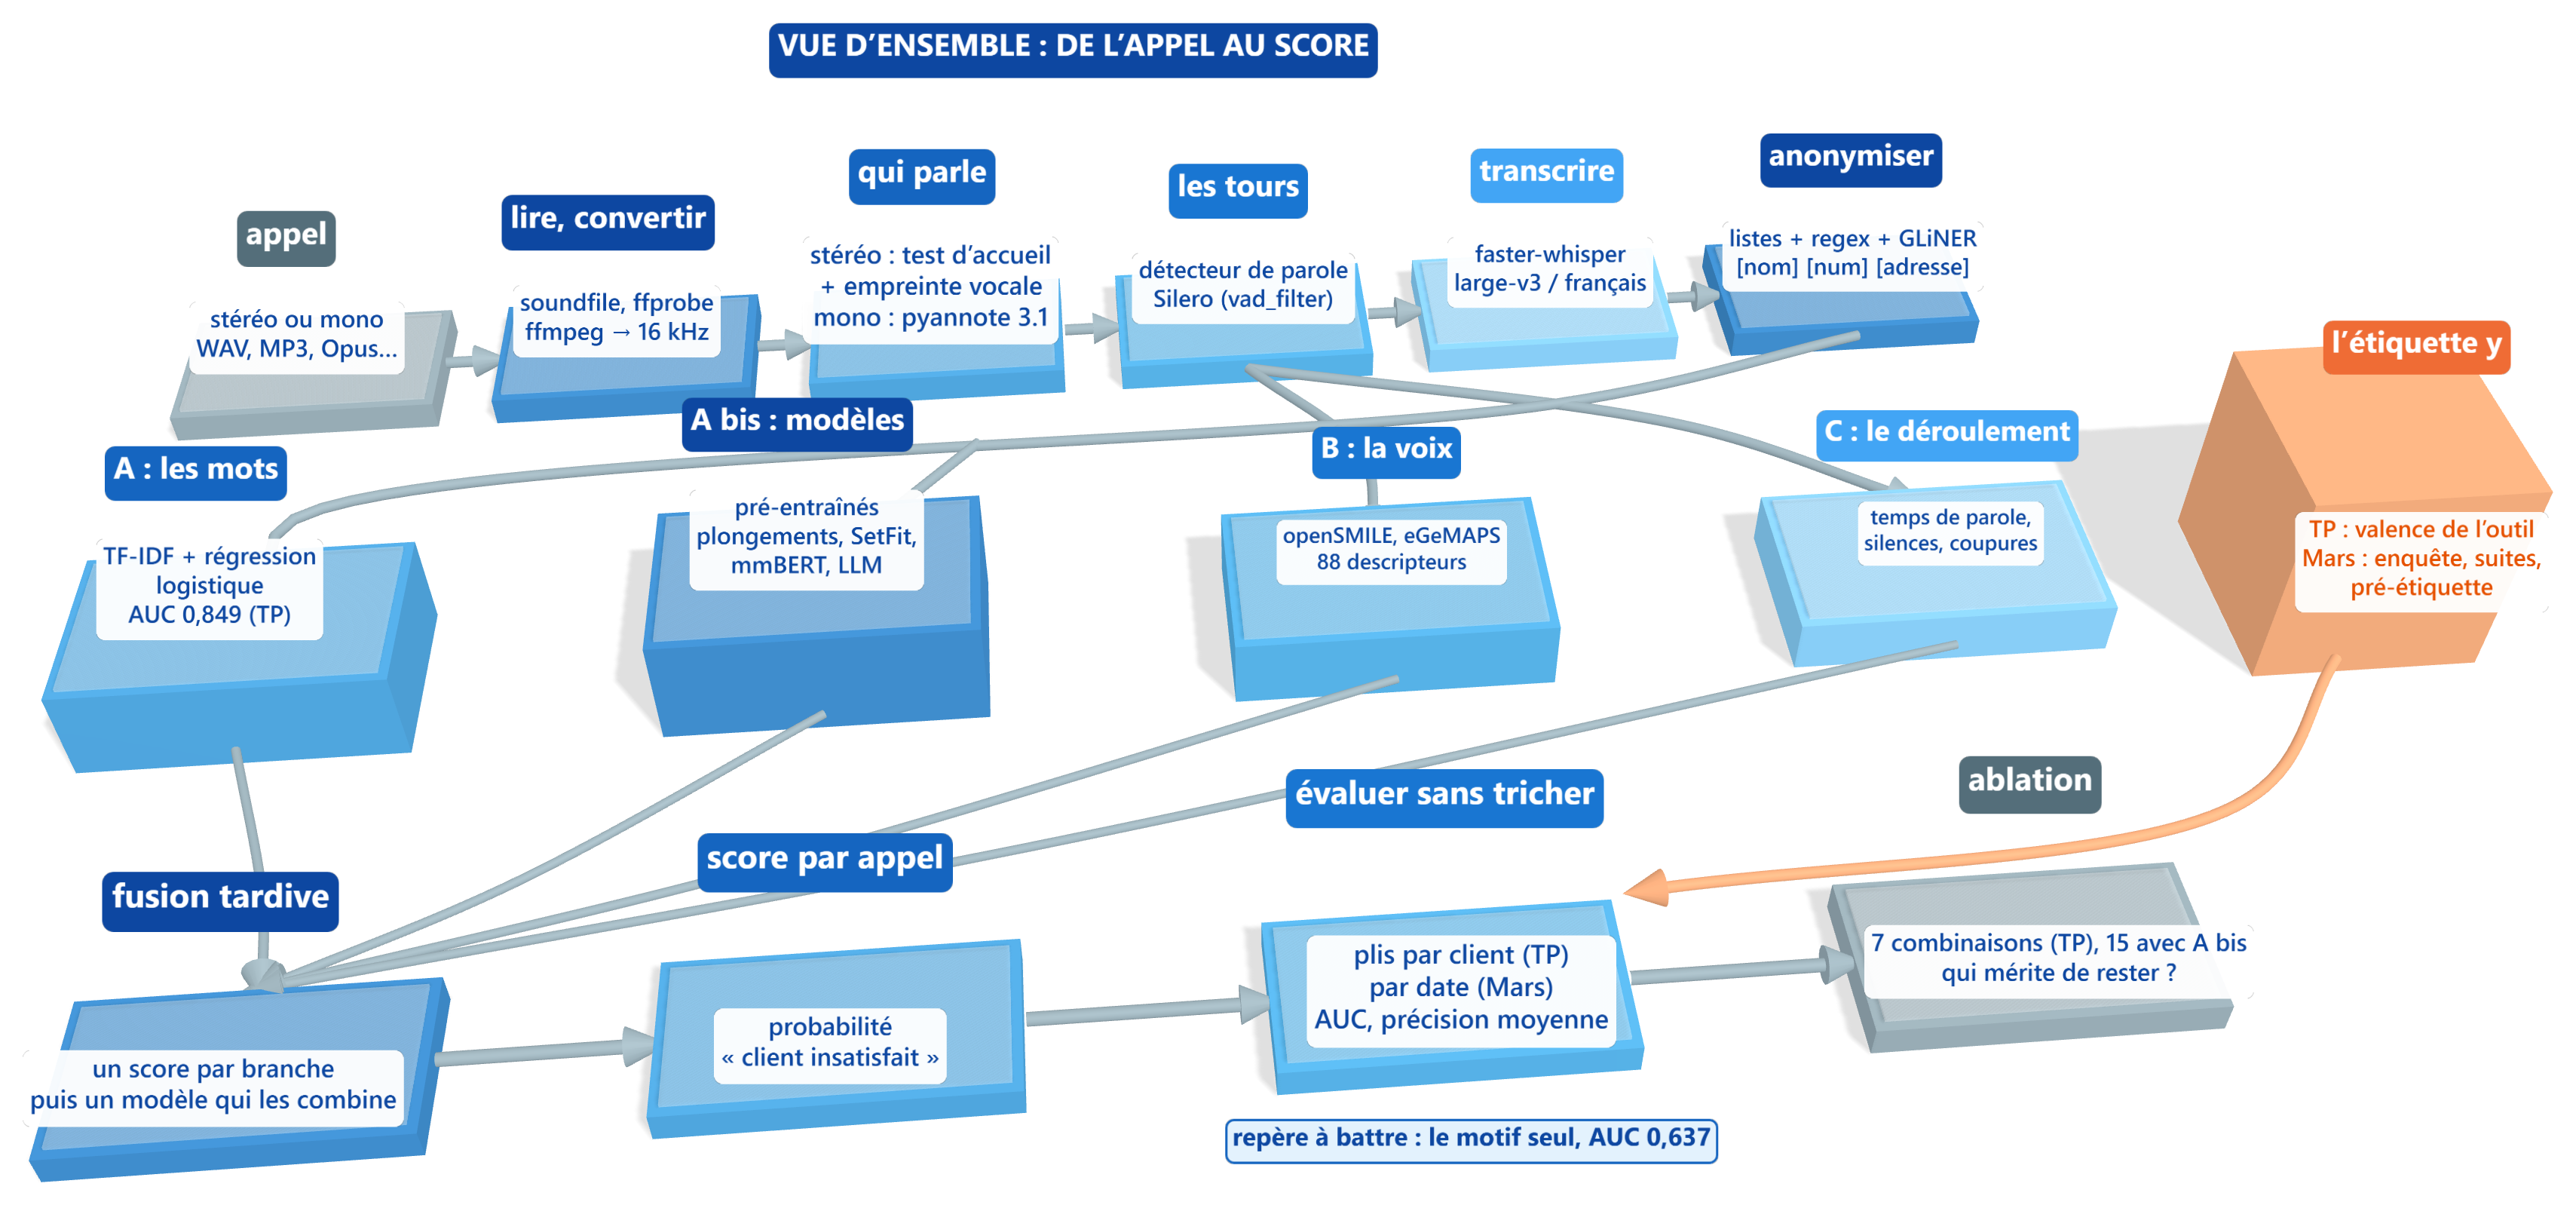
\includegraphics[width=\linewidth, height=12.2cm, keepaspectratio]{3d_ensemble.png}
\end{center}
\begin{tcbraster}[raster columns=3, raster equal height, raster column skip=6pt]
\begin{kpibox}[title={\faIcon{file-audio}\ 1. Préparer}, unbreakable]
\small Lire et convertir le son, savoir qui parle, découper les tours, transcrire, puis masquer noms et
numéros \textbf{avant tout modèle}.
\end{kpibox}
\begin{kpibox}[title={\faProjectDiagram\ 2. Des branches indépendantes}, unbreakable]
\small \textbf{A} les mots (TF-IDF), \textbf{A bis} les modèles pré-entraînés, \textbf{B} la voix,
\textbf{C} le déroulement : chacune donne un score, une fusion tardive les combine.
\end{kpibox}
\begin{kpibox}[title={\faBalanceScale\ 3. Juger honnêtement}, unbreakable]
\small Une étiquette auditée, un découpage sans tricher (par client, par date), un repère à battre
(0,637), puis l'ablation.
\end{kpibox}
\end{tcbraster}
\end{landscape}}

% Bandeau d'ouverture d'une grande partie
\newcommand{\bandeaupartie}[2]{\clearpage
\begin{tcolorbox}[colback=titlebg, colframe=titlebg, coltext=white, arc=5pt, boxrule=0pt,
  left=15pt, right=15pt, top=12pt, bottom=12pt]
\begin{center}{\Large\bfseries #1}\\[6pt]{\normalsize #2}\end{center}
\end{tcolorbox}}

\setlist[itemize]{leftmargin=1.5em, label={\color{sectioncolor}\textbullet}}
\setlist[enumerate]{leftmargin=1.5em, label={\color{sectioncolor}\arabic*.}}

% Page de titre commune : #1 sur-titre, #2 titre, #3 sous-titre, #4 ligne bleue, #5 objectif
\newcommand{\pagedetitre}[5]{%
\thispagestyle{empty}
\begin{tikzpicture}[remember picture, overlay]
  \fill[titlebg] (current page.north west) rectangle ([yshift=-8cm]current page.north east);
  \fill[lightblue] ([yshift=-8cm]current page.north west) rectangle ([yshift=-8.3cm]current page.north east);
  \fill[titlebg] (current page.south west) rectangle ([yshift=1.5cm]current page.south east);
  \fill[lightblue] ([yshift=1.5cm]current page.south west) rectangle ([yshift=1.8cm]current page.south east);
\end{tikzpicture}
\vspace*{0.1cm}
\begin{center}
  {\color{skyblue}\large\textbf{#1}}\\[0.5cm]
  {\color{white}\Huge\textbf{#2}}\\[0.4cm]
  {\color{palblue}\LARGE #3}\\[0.3cm]
  {\color{skyblue}\large #4}
\end{center}
\vspace*{1.6cm}
\begin{center}\couverture\end{center}
\vspace*{0.8cm}
\begin{center}
  \begin{tikzpicture}
    \node[fill=notebg, rounded corners=6pt, inner sep=14pt, text width=13cm, align=center,
      draw=sectioncolor, line width=0.8pt] {{\color{darkblue}\large\textbf{Objectif :} #5}};
  \end{tikzpicture}
\end{center}
\vfill
\begin{center}{\color{white}\small Année 2026--2027}\end{center}
\newpage
\setcounter{page}{1}}

% Illustration de couverture : le pipeline 1 en trois branches
\newcommand{\couverture}{%
\begin{tikzpicture}[
  b/.style={draw=##1, fill=##1!12, rounded corners=4pt, minimum width=3cm, minimum height=1.1cm,
    align=center, font=\small},
  a/.style={-{Stealth[length=2.5mm]}, thick, color=slate}]
\node[b=slate] (in) {{\Large\faPhone}\\Appel};
\node[b=darkblue, right=0.9cm of in] (d) {{\Large\faUsers}\\Qui parle ?};
\node[b=sectioncolor, right=0.9cm of d, yshift=1.5cm] (A) {{\Large\faFont}\\A : les mots};
\node[b=accentblue, right=0.9cm of d] (B) {{\Large\faWaveSquare}\\B : la voix};
\node[b=lightblue, right=0.9cm of d, yshift=-1.5cm] (C) {{\Large\faStopwatch}\\C : le rythme};
\node[b=darkblue, right=0.9cm of B] (out) {{\Large\faSmile\ \faFrown}\\Satisfait ?};
\draw[a] (in) -- (d); \foreach \x in {A,B,C} {\draw[a] (d) -- (\x); \draw[a] (\x) -- (out);}
\end{tikzpicture}}
